%\documentclass[xcolor=dvipsnames]{beamer} % dvipsnames gives more built-in colors
\documentclass[xcolor=dvipsnames,aspectratio=169,beamer]{beamer}
%\documentclass[xcolor=dvipsnames,aspectratio=169,handout]{beamer}
%\documentclass[xcolor=dvipsnames,handout]{beamer} 
\usepackage{pgfpages}
\usepackage[utf8]{inputenc} % für Umlaute ü, ä und ö

%%Sprachunterstuetzung
%Deutsche Silbentrennung, etc.
%\usepackage[ngerman]{babel}
\RequirePackage[english]{babel}
%Mehrsprachige Literaturliste
\usepackage{babelbib}

\usepackage{caption}
\usepackage{subcaption}
\usepackage{multimedia}
\usepackage{media9}
\usepackage{hyperref}
\usepackage{tabularx,booktabs}
\newcolumntype{L}[1]{>{\raggedright\let\newline\\\arraybackslash\hspace{0pt}}m{#1}}
\newcolumntype{C}[1]{>{\centering\let\newline\\\arraybackslash\hspace{0pt}}m{#1}}
\newcolumntype{R}[1]{>{\raggedleft\let\newline\\\arraybackslash\hspace{0pt}}m{#1}}

\graphicspath{{img/}{media/}} 
\addmediapath{media/}

\usepackage{beamerthemesplit}
\usepackage{lipsum}
\usetheme{Madrid}
\useoutertheme[subsection=false]{miniframes}
\useinnertheme{circles}
\newcommand{\backupbegin}{
   \newcounter{finalframe}
   \setcounter{finalframe}{\value{framenumber}}
}
\newcommand{\backupend}{
   \setcounter{framenumber}{\value{finalframe}}
}

\mode<beamer>{
\definecolor{UBCblue}{rgb}{0.417,0.582, 0.66}
\usecolortheme[named=UBCblue]{structure}
}
\mode<handout>{
\definecolor{UBCblue}{rgb}{0.417,0.582, 0.66}
\usecolortheme[named=UBCblue]{structure}
}
%\mode<handout>{
%\definecolor{UBCred}{rgb}{0.1, 0.8, 0.1}
%\usecolortheme[named=UBCred]{structure}
%}


\setbeamercovered{transparent=15}

\bibliographystyle{unsrtnat} 
\usepackage[sort&compress,numbers]{natbib}

%\usecolortheme[named=SkyBlue]{structure} % Sample dvipsnames color

\usepackage{amsmath, nccmath}
\setlength{\abovedisplayskip}{0pt}	

\usepackage{tikz} % graphics
\usepackage{tikz,pgfplots}

% Fancy Icons
\usepackage{fontawesome}

% Color definitions
\usepackage{xcolor}
\definecolor{color_red}{rgb}{1.0,0.0,0.0}%
\definecolor{color_blue}{rgb}{0.0,0.0,1.0}%

% Colored Box
%  Usage: \cfbox{red}
\newcommand{\cfbox}[2]{%
    \colorlet{currentcolor}{.}%
    {\color{#1}%
    \fbox{\color{currentcolor}#2}}%
}
\setlength{\fboxrule}{2pt}


\date{July 1, 2020}
\author{Silvio Emmenegger}
\institute[HSLU]{Final Presentation, Master Thesis FS20}
\title{Acoustic Scene and Room Classification for Real-Time Applications}

\usepackage{pgfpages}

%\setbeameroption{hide notes} % Only slides
%\setbeameroption{show only notes} % Only notes
%\setbeameroption{show notes on second screen=right}

%\setbeamerfont{framesubtitle}{size=\fontsize{20}{24}}

% Änderung Schriftgröße 
%\setbeamerfont{tiny structure}{size=\scriptsize}% alle Elemente mit beamerfont tiny structure 
%\setbeamerfont{headline}{size=\small}% alle Elemente mit beamerfont headline 
%\setbeamerfont{footline}{size=\small}% alle Elemente mit beamerfont footline 
\setbeamerfont*{subsection in head/foot}{size=\normalsize}


\newlength\SubHt
\settoheight\SubHt{\usebeamerfont{subsection in head/foot}S}
\newlength\SubDh
\settodepth\SubDh{\usebeamerfont{subsection in head/foot}g}

\makeatletter
\setbeamertemplate{headline}
{%
  \begin{beamercolorbox}[colsep=1.5pt]{upper separation line head}
  \end{beamercolorbox}
  \begin{beamercolorbox}{section in head/foot}
    \vskip2pt\insertnavigation{\paperwidth}\vskip2pt
  \end{beamercolorbox}%
  \ifbeamer@theme@subsection%
    \begin{beamercolorbox}[colsep=1.5pt]{middle separation line head}
    \end{beamercolorbox}
    \begin{beamercolorbox}[ht=1.5\SubHt,dp=2\SubDh,%defaults: ht=2.5ex,  dp=1.125ex
      leftskip=.3cm,rightskip=.3cm plus1fil]{subsection in head/foot}
      \usebeamerfont{subsection in head/foot}\insertsubsectionhead
    \end{beamercolorbox}%
  \fi%
  \begin{beamercolorbox}[colsep=1.5pt]{lower separation line head}
  \end{beamercolorbox}
}
\makeatother


\makeatletter
\setbeamertemplate{footline}
{
  \leavevmode%
  \hbox{%
  \begin{beamercolorbox}[wd=.333333\paperwidth,ht=2.25ex,dp=1ex,center]{author in head/foot}%
    \usebeamerfont{author in head/foot}\insertauthor \space (HSLU)
  \end{beamercolorbox}%
  \begin{beamercolorbox}[wd=.333333\paperwidth,ht=2.25ex,dp=1ex,center]{title in head/foot}%
    \usebeamerfont{title in head/foot}Master Thesis
  \end{beamercolorbox}%
  \begin{beamercolorbox}[wd=.333333\paperwidth,ht=2.25ex,dp=1ex,right]{date in head/foot}%
    \usebeamerfont{date in head/foot}\insertshortdate{}\hspace*{2em}
    \insertframenumber{} / \inserttotalframenumber\hspace*{2ex} 
  \end{beamercolorbox}}%
  \vskip0pt%
}
\makeatother


\begin{document}
	
  \mode<beamer>{
  \bgroup
  \makeatletter
  \setbeamertemplate{footline} 
  {
    \leavevmode%
    \hbox{%
  
    \begin{beamercolorbox}[wd=.333333\paperwidth,ht=2.25ex,dp=1ex,center]
    {author in head/foot}%
    \usebeamerfont{author in head/foot}\insertauthor \space (HSLU)
    \end{beamercolorbox}%
  
    \begin{beamercolorbox}[wd=.333333\paperwidth,ht=2.25ex,dp=1ex,center]
    {title in head/foot}%
      \usebeamerfont{title in head/foot}
      Master Thesis
    \end{beamercolorbox}%
  
    \begin{beamercolorbox}[wd=.333333\paperwidth,ht=2.25ex,dp=1ex,right]
      {date in head/foot}%
      \usebeamerfont{date in head/foot}\insertshortdate{}\hspace*{2em}
      %\insertframenumber{} / \inserttotalframenumber\hspace*{2ex} 
    \end{beamercolorbox}}%
  
    \vskip0pt%
  }
  \makeatother
  \begin{frame}
  \vspace{20mm}
  \titlepage
  \end{frame}
  \egroup
  }
  \addtocounter{framenumber}{-1}
	
	
%%%%%%%%%%%%%%%%%%%%%%%%%%%%%%%%%%%%%%%%%%%%%%%%%%%%%%%%%%%%%
	
\section{Motivation}

\begin{frame}
	\centering
	\begin{flushleft}
		\huge{Acoustic environments in daily life}	
	\end{flushleft}
	
	\begin{figure}[htb!]
	\cfbox{white}{
	\begin{minipage}[t]{0.28\textwidth}
	  \centering
      \includemedia[
		addresource=00124_02-01_livingroom-music.mp3,
		flashvars={
   			source=00124_02-01_livingroom-music.mp3
				   &autoPlay=true
  			}
  	  ]{\scriptsize\fbox{\faPlay \hspace{1mm} Play}}{APlayer.swf}	
  	  \\
  	  \vspace{2mm}
	  {
	  	\scriptsize\textbf{Livingroom/Music}
	  } \\ 
	  \tiny Lucerne, Home \\ \vspace{1mm}
	  
	  \includegraphics[width=1.0\textwidth]{01_Sample_Livingroom_Lucerne.png}		  
	\end{minipage}
	}
	\cfbox{white}{
	\begin{minipage}[t]{0.28\textwidth}
		Column 2
	\end{minipage}	
	}
	\hspace{-2.5mm}
	\cfbox{white}{
	\begin{minipage}[t]{0.28\textwidth}
		Column 2	
	\end{minipage}	
	\hspace{-2.5mm}
	}
	\end{figure}
	
%	\vspace{3mm}
	\begin{flushleft}
	{\tiny 
		Sources: 
		https://bit.ly/31p4k32
	}	
	\end{flushleft}
	
\end{frame}


\begin{frame}[t]

	\textbf{Intention}
	\begin{itemize}
	\item<1-> Creation of acoustic classifier system for scenes and soundscapes
	\item<2-> Classification at the edge in real-time $\rightarrow$ hearing aids
	\item<3-> Use of latest AI techniques $\rightarrow$ Convolutional Neural Networks (CNN)
	\end{itemize}
	
\end{frame}

\section{Introduction}

\begin{frame}
	\textbf{Tasks}
	\begin{itemize}
	\item<1-> Record new audio dataset and labels with high-quality equipment
	\item<2-> Preprocessing of audio into image-like features
	\item<3-> Train CNN model on created feature dataset
	\item<4-> Optimize CNN model with simple grid search method
	\item<5-> Propose real-time implementation concept for dedicated hardware
	\end{itemize}
	\vspace{5mm}
	\only<1>{
		\hspace{10mm}
		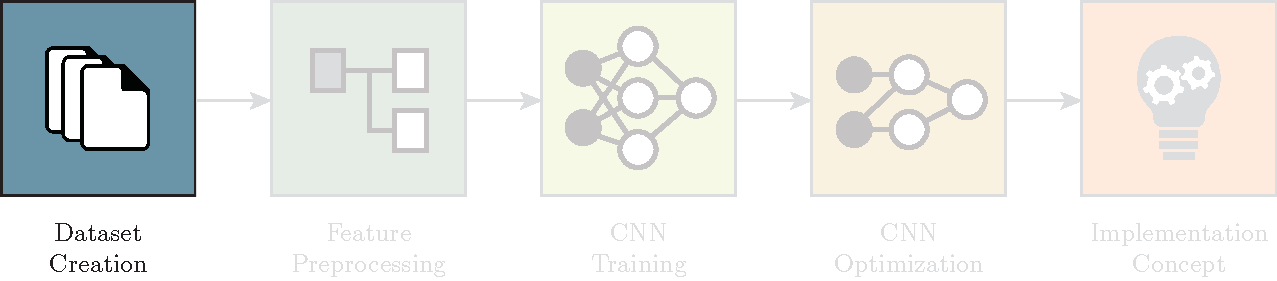
\includegraphics[width=0.85\textwidth]{03_Concept_Overview_1.pdf}
	}
	\only<2>{
		\hspace{10mm}
		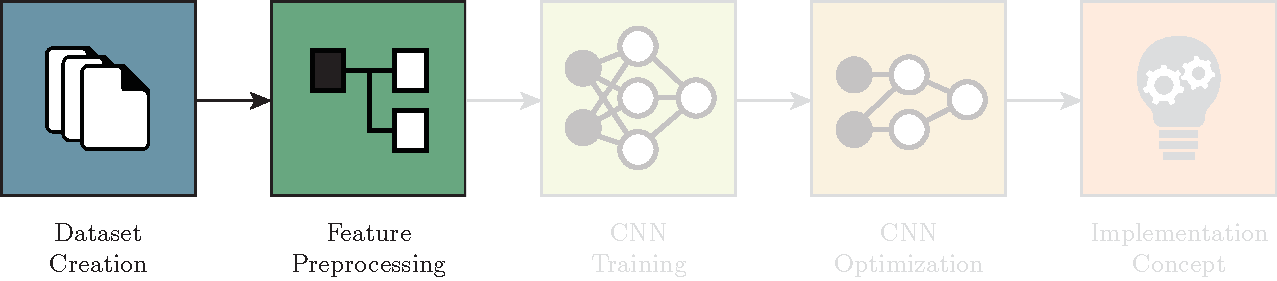
\includegraphics[width=0.85\textwidth]{03_Concept_Overview_2.pdf}
	}
	\only<3>{
		\hspace{10mm}
		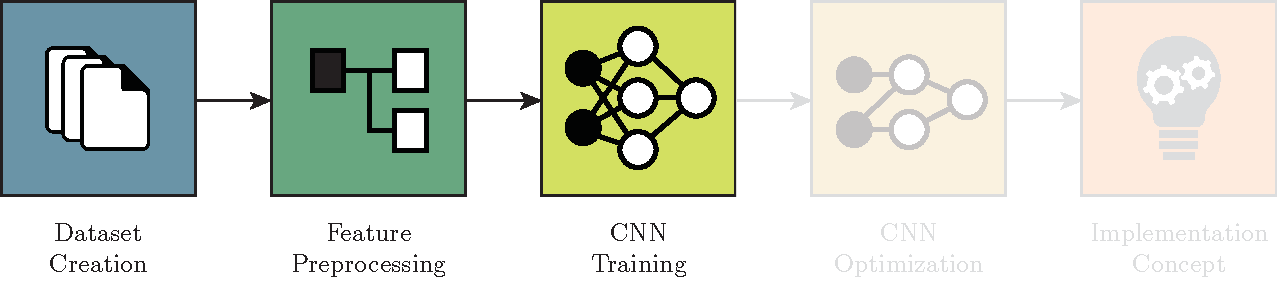
\includegraphics[width=0.85\textwidth]{03_Concept_Overview_3.pdf}
	}
	\only<4>{
		\hspace{10mm}
		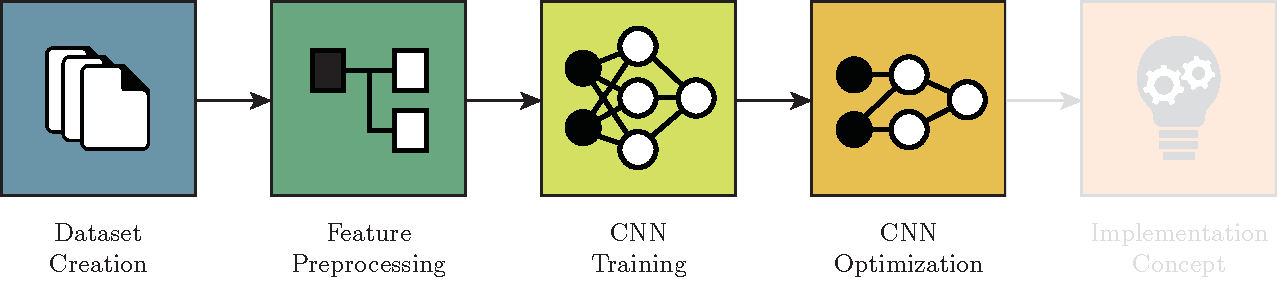
\includegraphics[width=0.85\textwidth]{03_Concept_Overview_4.pdf}
	}
	\only<5>{
		\hspace{10mm}
		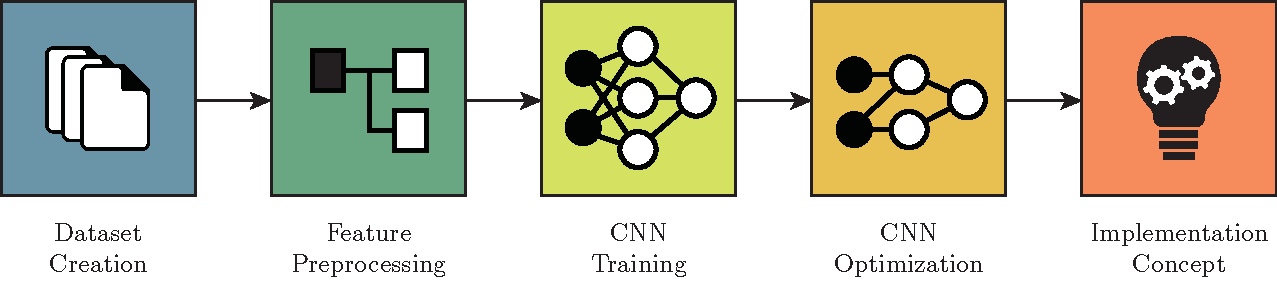
\includegraphics[width=0.85\textwidth]{03_Concept_Overview_5.pdf}
	}
\end{frame}

\section{Concept \& Realization}

\begin{frame}
	\textbf{Dataset Creation}
	\begin{itemize}
	\item<1-> Two labels with five classes each (\glqq{}2D\grqq{} label combinations)
	\item<2-> Multi-class multi-output classification problem, supervised
	\item<3-> Binaural recordings with $f_s=48$ kHz and 16-bit quantization learning
	\item<4-> At least 60 min for each label combination $\rightarrow$ 25h in total
	\end{itemize}
	
	\begin{flushleft}
	\begin{minipage}{0.6\textwidth}
	
	\vspace{5mm}
	\begin{minipage}{0.47\textwidth}
	\begin{table}[h!]
		\small
    	\raggedleft
		\begin{tabular}{C{3cm}} 
    	\toprule
		Scenes \\
		\midrule
		Cafeteria/Canteen \\
		Car (inside) \\
		Livingroom \\
		Nature \\
		Street \\
		\bottomrule
		\end{tabular}
	\end{table}
	\end{minipage}
	\hspace{2mm}
	\begin{minipage}{0.47\textwidth}
	\begin{table}[h!]
		\small
    	\raggedright
		\begin{tabular}{C{3cm}} 
    	\toprule
		Soundscapes \\
		\midrule
		Music \\
		Noise \\
		Speech \\
		Noisy Speech \\
		Quiet \\		
		\bottomrule
		\end{tabular}
	\end{table}
	\end{minipage}
	
	\end{minipage}
	\begin{minipage}{0.38\textwidth}
	  \centering
	  \only<1-2>{
		  
\includegraphics[width=0.95\textwidth]{04_Recording_Equipment_white.pdf}
	  }
	  \only<3->{
		  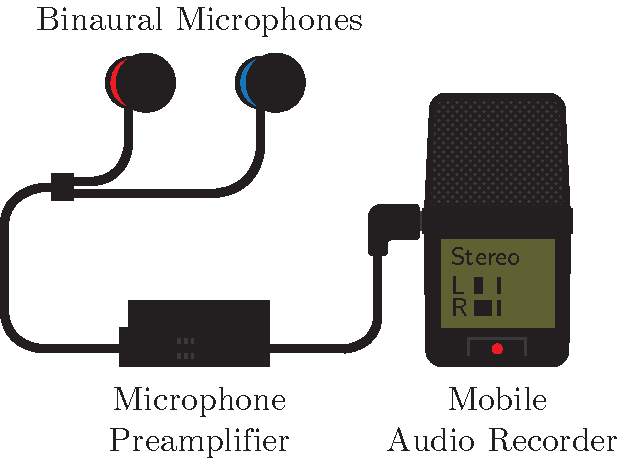
\includegraphics[width=0.95\textwidth]{04_Recording_Equipment.pdf}
	  }
	\end{minipage}	
	\end{flushleft}

\end{frame}	


\section{Results}


\section{Demonstration}
\begin{frame}

	\begin{center}
	\only<1>{
	\huge Demonstrator
	}
	\only<2>{
	\huge Questions $\&$ Discussion
	}
	\end{center}

\end{frame}	


\appendix
\backupbegin

\section{Backup Slides}
\begin{frame}

	\begin{center}
	\textbf{Backup Slides}
	\end{center}

\end{frame}	

\begin{frame}

   	\addcontentsline{toc}{section}{Bibliography}
	\textbf{Bibliography}
	{\small
		\bibliography{references}
	}

\end{frame}


\section{Backup Slides}


\begin{frame}

	\textbf{Backup Slides 1}	
	Ref. \cite{bib:fischer}
		
\end{frame}

\backupend

\end{document}